\documentclass[xcolor=dvipsname]{beamer}

%\usepackage[ngerman]{babel}
\usepackage[T1]{fontenc}
\usepackage[utf8]{inputenc}
\usepackage{amsmath}
\usepackage{graphicx}
\usepackage{subfigure}
\usepackage{multimedia}
\usepackage{wrapfig}
\usepackage{listings}
\usepackage{comment}
\usepackage{framed,color}

\fboxsep=1pt%padding thickness
\fboxrule=1pt%border thickness
\usepackage{fancybox}

\usepackage{lipsum}
\usepackage{tabularx}
\usepackage{colortbl}
\usepackage{url}


\hypersetup{
	linkcolor=DarkSkyBlue,
	citecolor= DarkSkyBlue,
	filecolor= DarkSkyBlue,
	urlcolor= DarkSkyBlue
}


% COLOR-DEFINITION
%%%%%%%%%%%%%%%%%%%%%%%%
\definecolor{LightButter}{rgb}{0.98,0.91,0.31}
\definecolor{LightOrange}{rgb}{0.98,0.68,0.24}
\definecolor{LightChocolate}{rgb}{0.91,0.72,0.43}
\definecolor{LightChameleon}{rgb}{0.54,0.88,0.20}
\definecolor{LightSkyBlue}{rgb}{0.45,0.62,0.81}
\definecolor{LightPlum}{rgb}{0.68,0.50,0.66}
\definecolor{LightScarletRed}{rgb}{0.93,0.16,0.16}
\definecolor{LightGray}{rgb}{0.80,0.80,0.80}
\definecolor{Butter}{rgb}{0.93,0.86,0.25}
\definecolor{Orange}{rgb}{0.96,0.47,0.00}
\definecolor{Chocolate}{rgb}{0.75,0.49,0.07}
\definecolor{Chameleon}{rgb}{0.45,0.82,0.09}
\definecolor{SkyBlue}{rgb}{0.20,0.39,0.64}
\definecolor{Plum}{rgb}{0.46,0.31,0.48}
\definecolor{ScarletRed}{rgb}{0.80,0.00,0.00}
\definecolor{DarkButter}{rgb}{0.77,0.62,0.00}
\definecolor{DarkOrange}{rgb}{0.80,0.36,0.00}
\definecolor{DarkChocolate}{rgb}{0.56,0.35,0.01}
\definecolor{DarkChameleon}{rgb}{0.30,0.60,0.02}
\definecolor{DarkSkyBlue}{rgb}{0.12,0.29,0.53}
\definecolor{DarkPlum}{rgb}{0.36,0.21,0.40}
\definecolor{DarkScarletRed}{rgb}{0.64,0.00,0.00}



% HPI-THEME
%%%%%%%%%%%%%%%%%%%%%%%%
\RequirePackage{scrlfile}
%\ReplaceFile{beamerthemehpiswa.sty}{theme/beamerthemehpiswa.sty}
%\ReplaceFile{beamercolorthemehpiswa.sty}{theme/beamercolorthemehpiswa.sty}
%\ReplaceFile{beamerfontthemehpiswa.sty}{theme/beamerfontthemehpiswa.sty}
%\ReplaceFile{beamerinnerthemehpiswa.sty}{theme/beamerinnerthemehpiswa.sty}
%\ReplaceFile{beamerouterthemehpiswa.sty}{theme/beamerouterthemehpiswa.sty}
%\ReplaceFile{hpi.png}{theme/hpi.png}
\usetheme{hpiswa}


% BEAMER-Anpassungen
%%%%%%%%%%%%%%%%%%%%%%%%
\setbeamercolor{block title}{bg=DarkOrange}
\setbeamercolor{block body}{bg=Orange!20}
%\setbeamercolor{block title alerted}{bg=red}
\setbeamercolor{block body alerted}{bg=red!20}
%\setbeamercolor{block title example}{bg=green}
\setbeamercolor{block body example}{bg=DarkChameleon!20}
%\usecolortheme[RGB={205,173,0}]{structure}
\usecolortheme[RGB={30,74,135}]{structure}

\usecolortheme{orchid}
%\usefonttheme{professionalfonts}
%\useoutertheme[subsection=false]{smoothbars}
%\useinnertheme{rectangles}
%\setbeamertemplate{blocks}[shadow=true]

\setbeamercovered{transparent}
\setbeamertemplate{navigation symbols}{}%remove navigation symbols



% Eigene Anpassungen
%%%%%%%%%%%%%%%%%%%%

\definecolor{javared}{rgb}{0.6,0,0} % for strings
\definecolor{javagreen}{rgb}{0.25,0.5,0.35} % comments
\definecolor{javapurple}{rgb}{0.5,0,0.35} % keywords
\definecolor{javadocblue}{rgb}{0.25,0.35,0.75} % javadoc

\lstset{
  language=Java,
  basicstyle=\scriptsize\ttfamily,
  keywordstyle=\color{javapurple}\bfseries,
  stringstyle=\color{javared},
  commentstyle=\color{javagreen},
  morecomment=[s][\color{javadocblue}]{/**}{*/},
  tabsize=4,
  showspaces=false,
  showstringspaces=false,
  breaklines=true
}

% Explainframes:
\usepackage{ifthen}
\newboolean{isexplainframe}
\setboolean{isexplainframe}{false}
\mode<handout>{
\newenvironment{explainframe}[1]{
\setboolean{isexplainframe}{true}
\addtocounter{framenumber}{-1}
\setbeamertemplate{background}[grid][step=5mm,color=LightGray]
\begin{frame}{Handout only: #1}%
}{%
\end{frame}%
\setboolean{isexplainframe}{false}
}}
\mode<beamer>{
\excludecomment{explainframe}
}

\setbeamertemplate{footline}{%
	\leavevmode%
	\hbox{%
		\begin{beamercolorbox}[wd=.45\paperwidth,ht=2.25ex,dp=1ex,center]{author in head/foot}%
			\usebeamerfont{author in head/foot}\insertinstitute
		\end{beamercolorbox}%
		\begin{beamercolorbox}[wd=.2\paperwidth,ht=2.25ex,dp=1ex,center]{title in head/foot}%
			\usebeamerfont{title in head/foot}\insertshorttitle
		\end{beamercolorbox}%
		\begin{beamercolorbox}[wd=.45\paperwidth,ht=2.25ex,dp=1ex,right]{date in head/foot}%
			\usebeamerfont{date in head/foot}\insertshortdate{}\hspace*{2em}
			\insertframenumber{}\ifthenelse{\boolean{isexplainframe}}{E}{} / \inserttotalframenumber\hspace*{2ex}
	\end{beamercolorbox}}%
	\vskip0pt%
}


% Gliederung vor jedem Punkt:
\AtBeginSection[]{
\ifthenelse{\equal{\value{section}}{1}}{}{
\begin{frame}{Overview}
	\tableofcontents[currentsection, hideothersubsections]
\end{frame}
}
}


% Quote-Environment:

\renewenvironment{quote}{%
\begin{exampleblock}{}%
\begin{center}%
\begin{large}%
``}{%
''\end{large}%
\end{center}%
\end{exampleblock}}


\newcommand{\idea}[1]{$\rightarrow$ #1}



% Dokument-Meta-Daten:
%%%%%%%%%%%%%%%%%%%%%%%
\title{Truffle}
\subtitle{Virtual Machines and Execution Environments, WS2014/15}
\author{Jan Graichen, Fabio Niephaus, Matthias Springer, Malte Swart}
\date{\today}
\institute[2012]{Hasso Plattner Institute, Software Architecture Group}



\begin{document}

\begin{frame}[plain]
	\maketitle
\end{frame}
\begin{frame}{Overview}
	\tableofcontents[hideallsubsections]
\end{frame}

\section{How to implement a programming language?}

\begin{frame}{How to implement a programming language?}
    \begin{enumerate}
        \item Prototype your language: build an abstract syntax tree (AST) interpreter \\
        easy to implement, but slow (tree traversal, virtual method calls)
        \item Make it fast: build a VM, compile AST to byte code, JIT compilation \\
        hard to implement, reinvent the wheel (memory management etc.)
    \end{enumerate}

    \vfill
    \begin{alertblock}{With Truffle}
        Truffle: ``how it should be''. Build a parser, define an AST, and add language specific optimizations make it fast.
    \end{alertblock}
\end{frame}


\section{How it works}

\begin{frame}{Infrastructure}
	\begin{figure}
        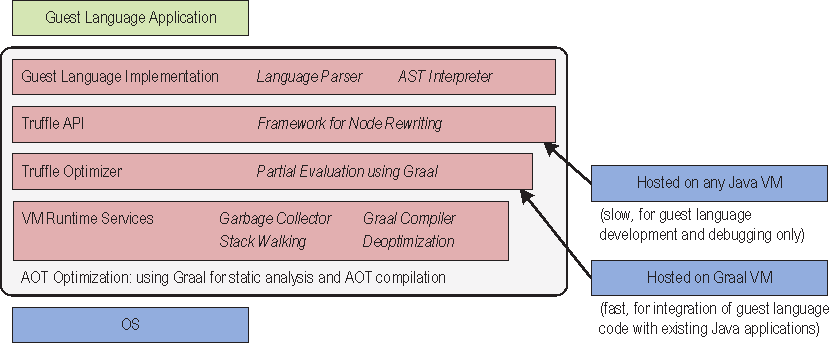
\includegraphics[width=\textwidth]{infrastructure.pdf}
        \caption{Interaction Graal/Truffle}
        \label{fig:interaction}
    \end{figure}
\end{frame}

\begin{explainframe}{Infrastructure}
	\begin{itemize}
    	\item Main components
        \begin{itemize}
            \item Truffle: provides guest language implementation API, support for optimization through node rewriting
        	\item Graal VM: HotSpot VM with Java API (instructured by Truffle)
        \end{itemize}
    	\item Two levels of optimization: Truffle, modified Graal VM
    \end{itemize}
\end{explainframe}

\begin{frame}[fragile]{Truffle: How it works}
	\begin{itemize}
    	\item Truffle: AST Interpreter Framework
        \item Framework to easily implement specialized nodes
        \item Supports AST node rewriting
    \end{itemize}

       \vfill
       \pause
        \begin{block}{Sample Code}
    	\begin{lstlisting}
        function add(a, b) {
        	return (a + b) + " ms";
        }
      \end{lstlisting}
	\end{block}
\end{frame}

\begin{frame}[fragile]
    \frametitle{Node Rewriting}
	\begin{figure}
    	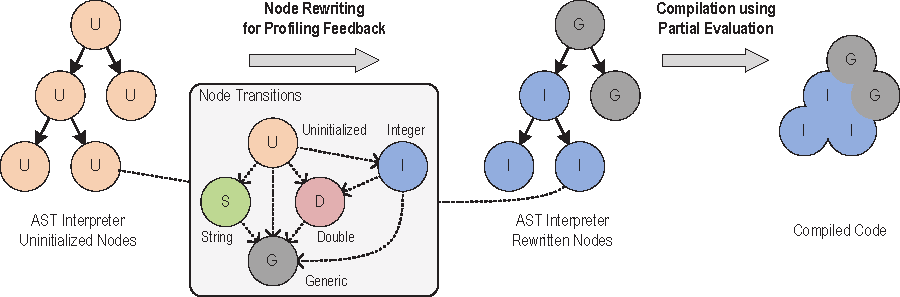
\includegraphics[width=\textwidth]{node_rewriting.pdf}
        \caption{Node Rewriting Example}
        \label{fig:node_rewriting}
    \end{figure}

    \begin{block}{Sample Code}
   	\begin{lstlisting}
        add(1, 2);
    \end{lstlisting}
    \end{block}
\end{frame}

\begin{explainframe}{Node Rewriting}
    \begin{itemize}
        \item Generic nodes can handle all types.
        \item Guards check if the type specialization is still accurate.
        \item Partial evaluation once a tree stablized (no rewrites for a while) and is \emph{hot}.
        \begin{itemize}
        	\item Inlines \texttt{execute()} methods generates native code.
            \item Adds a check and a deoptimization call where a rewrite could happen.
        	\item Requires Graal (accessing compiler with Java code).
        \end{itemize}
        \item Truffle without Graal: interpreter mode
    \end{itemize}
\end{explainframe}

\begin{frame}[fragile]{Deoptimization}
    \begin{figure}
        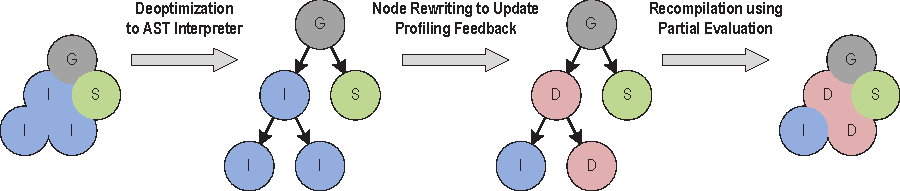
\includegraphics[width=\textwidth]{deopt.pdf}
        \caption{Deoptimization of Native Code}
        \label{fig:deopt}
    \end{figure}
    \begin{block}{Sample Code}
    	\begin{lstlisting}
      add(1, 2.5);
      \end{lstlisting}
	\end{block}
\end{frame}

% Boxing Elimination, Tree Cloning

\begin{frame}[fragile]{Code example (unoptimized)}
\begin{lstlisting}
public Object add(...) {
  Object left = leftNode.executeGeneric(...);
  Object right = rightNode.executeGeneric(...);

  if (left instanceof Long && right instanceof Long) {
    try {
      return ExactMath.addExact((Long) left, (Long) right);
    } catch (ArithmeticException ex) { }
  }

  if (left instanceof Long)
      left = ((Long) left).doubleValue();
  if (right instanceof Long)
      right = ((Long) right).doubleValue();

  if (left instanceof Double && right instanceof Double)
    return (Double) left + (Double) right;

  if (left instanceof String || right instanceof String)
    return left.toString() + right.toString();

  throw new UnsupportedSpecializationException(...);
}
\end{lstlisting}
\end{frame}

\begin{frame}[fragile]{Code example using annotation-based DSL}
  \begin{lstlisting}
public abstract class SLAddNode extends SLBinaryNode {
  @Specialization(rewriteOn=ArithmeticException.class)
  protected final long add(long left, long right) {
    return ExactMath.addExact(left, right);
  }

  @Specialization
  protected final double add(double left, double right) {
    return left + right;
  }

  @Specialization(guards = "isString")
  protected final String add(Object left, Object right) {
    return left.toString() + right.toString();
  }

  protected final boolean isString(Object a, Object b) {
    return a instanceof String || b instanceof String;
  }
}
  \end{lstlisting}
\end{frame}

\begin{frame}{Code example using annotation-based DSL}

	    \begin{figure}
        \centering
        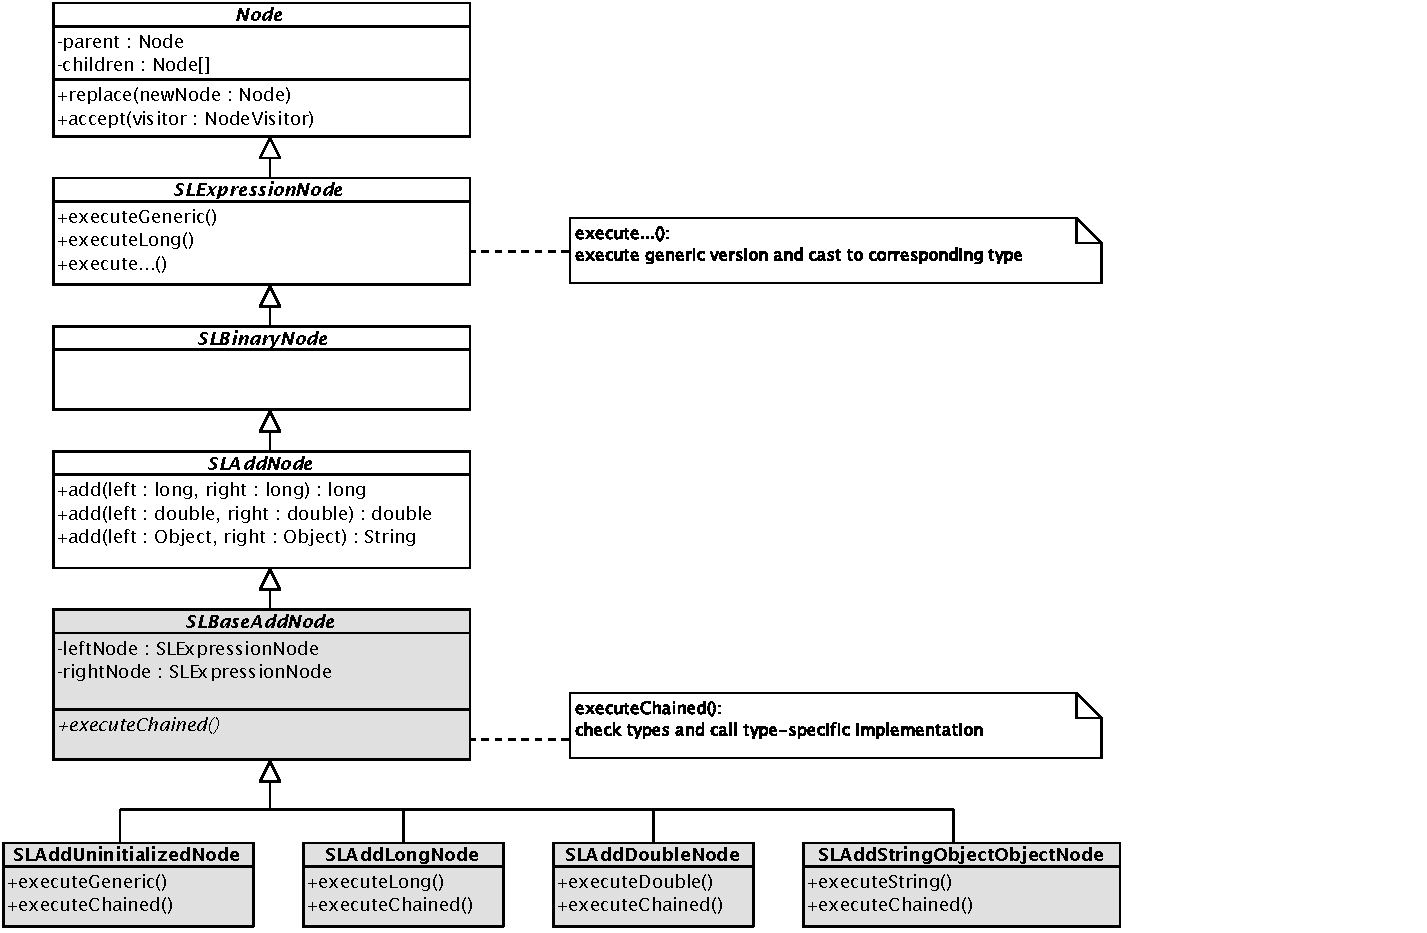
\includegraphics[width=0.8\textwidth]{nodes_less.pdf}
        \caption{Generated classes for code example}
        \label{fig:gencodes}
    \end{figure}

\end{frame}

\begin{explainframe}{Code example}
	\begin{itemize}
    	\item Defined by language implementor: \\ \lstinline{SLExpressionNode}, \lstinline{SLBinaryNode}, \lstinline{SLAddNode}
        \item Generic case is generated by preprocessor
        \item \textbf{Uninitialized node:} replaces itself with specialized node
        \item \textbf{Monomorphic node:} one specialization only
        \item \textbf{Megamorphic node:} node can handle all types \\ (last item on linked list)
    \end{itemize}
\end{explainframe}

\section{Optimizations}
%%%%%%%%%%%%%%%%%%%%%%%%%

\subsection{Node rewriting}
% Self
\begin{frame}[fragile]{AST rewriting}
    \begin{block}{JavaScript}
   	\begin{lstlisting}
function foo() {
    return add(1, 2) + add("hello", "world");
}

function add(a, b) {
    return a + b;
}
    \end{lstlisting}
    \end{block}
\end{frame}

\begin{frame}[fragile]{AST inlining}
  \begin{figure}
    \centering
    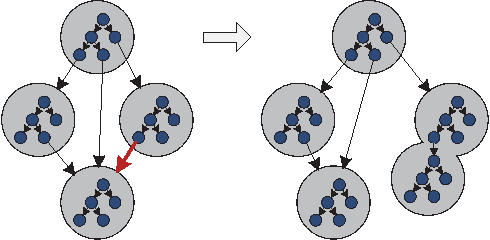
\includegraphics[width=0.8\textwidth]{image02-2.pdf}
    \caption{AST inlining}
    \label{fig:inlining}
  \end{figure}
\end{frame}

\begin{frame}[fragile]{AST inlining}
  \begin{figure}
    \centering
    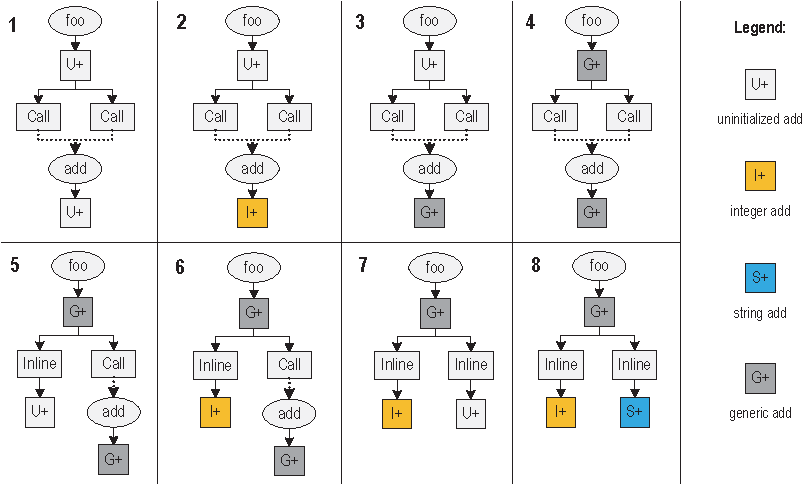
\includegraphics[width=0.8\textwidth]{image01-2.pdf}
    \caption{AST evolution}
    \label{fig:inlining2}
  \end{figure}
\end{frame}

\begin{frame}{Polymorphic Inline Caching}
  \begin{figure}
    \centering
    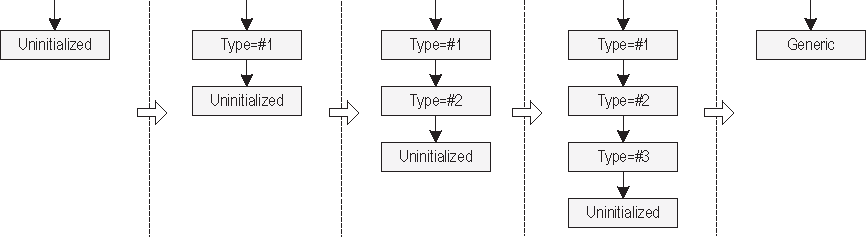
\includegraphics[width=0.9\textwidth]{poly.pdf}
    \caption{Polymorphic AST Nodes}
    \label{fig:poly}
  \end{figure}
\end{frame}

\begin{frame}{Polymorphic Inline Caching}
  \begin{figure}
    \centering
    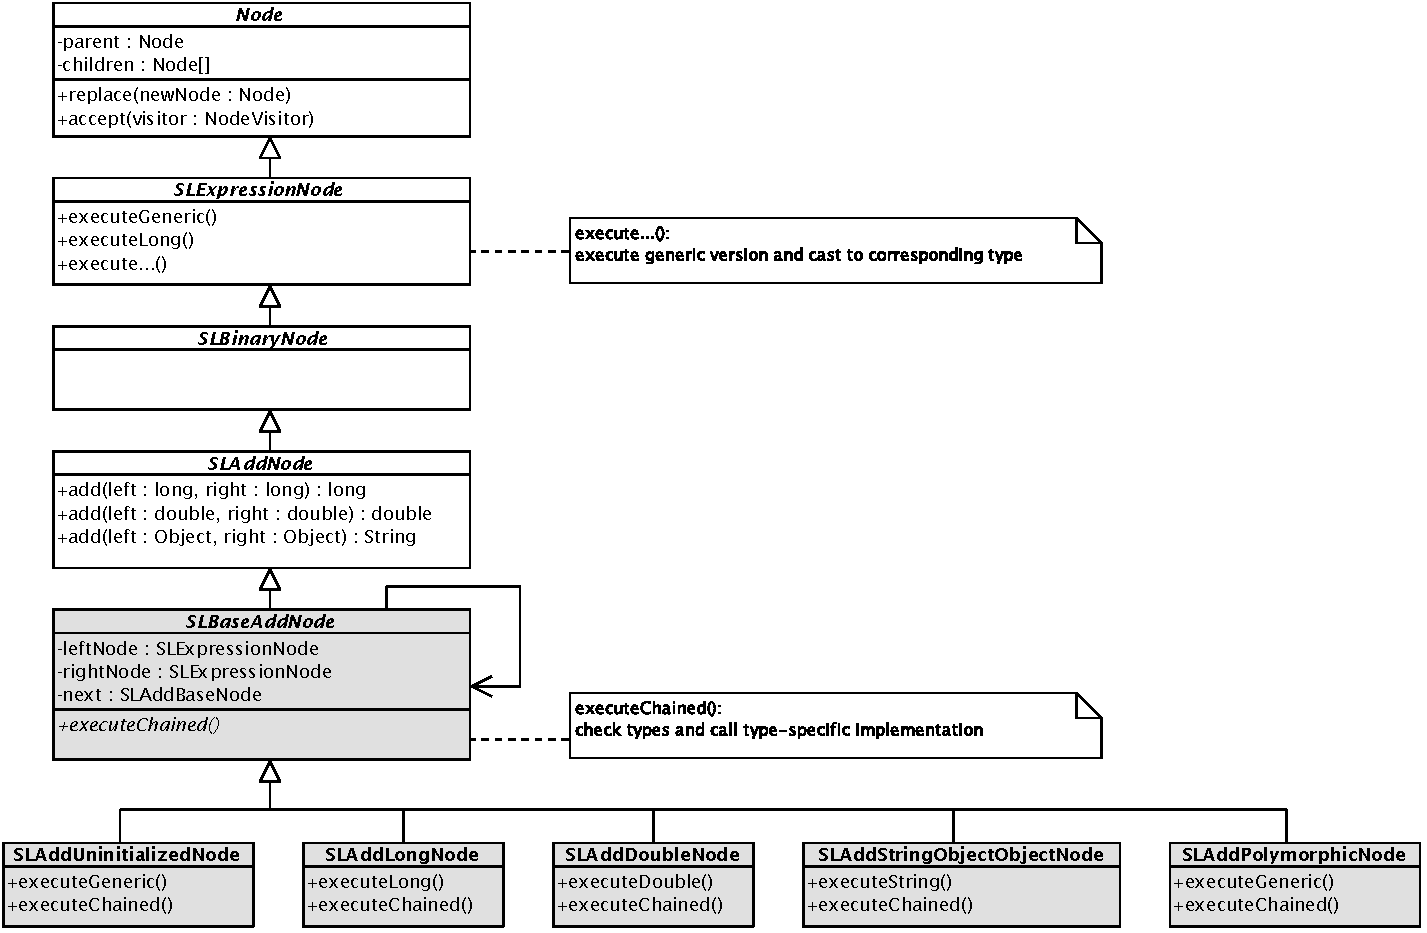
\includegraphics[width=0.8\textwidth]{nodes.pdf}
    \caption{Generated classes for code example}
  \end{figure}
\end{frame}

\begin{explainframe}{Polymorphic Inline Caching}
    \begin{itemize}
        \item \textbf{Polymorphic node:} node can handle a limited set of types (linked list via \lstinline{next} field): polymorphic inline caching
        \item Last element in linked list is megamorphic
    \end{itemize}
\end{explainframe}

\subsection{Assumptions}
\begin{frame}{Assumptions}
    \begin{alertblock}{Requirement}
        Global assumptions about system state, like:
        \begin{itemize}
          \item Redefinition of system objects or methods (JavaScript, Ruby)
          \item Current class hierarchy (Java)
        \end{itemize}
    \end{alertblock}
    \pause
    \vfill
    \begin{itemize}
        \item Global one-time switch; bool can be changed to \lstinline{false} once
        \pause
        \item Partial evaluation with constant value instead of check
        \pause
        \item On state change code is deoptimized
    \end{itemize}
    \pause
    \begin{center}
        \alert{No runtime overhead in compiled code}
    \end{center}
\end{frame}
\begin{frame}[fragile]{Example: Assumption for method redefinition}
  \begin{lstlisting}
final class MyCallNode {
  private final MyFunction function;
  private final Assumption functionStable;

  protected SLDirectDispatchNode(...MyFunction function) {
    this.function = function;
    this.functionStable = function.getStableAssumption();
  }

  protected Object execute(...) {
    try {
      functionStable.check();
      return function.call(...);
    } catch(InvalidAssumptionException ex) {
      replace(...);
    }
  }
}
  \end{lstlisting}
\end{frame}

\subsection{Local variables}
\begin{frame}{Local variables}
    \begin{alertblock}{Requirement}
        Highly efficient local variables access while simple modeling
        \begin{itemize}
          \item Modeled as an array on \texttt{Frame} object
          \item Access nodes must be specializable for dynamic profiling
        \end{itemize}
    \end{alertblock}
    \pause
    \vfill
    \begin{itemize}
        \item Escape analysis of local variable array access
        \pause
        \item Implicit single static assignment (SSA) form
        \pause
        \item Host compiler can optimize without flow analysis
        \pause
        \item \texttt{Frame} array never allocated except on deoptimization
    \end{itemize}
    \pause
    \begin{center}
        \alert{As fast as host language variables; optional  \texttt{Frame} facilities}
    \end{center}
\end{frame}

\begin{frame}[fragile]{Single static assignment (SSA) form}
  \begin{block}{Source example}
  \begin{lstlisting}
if(condition) {
  x = value1 + value2;
} else {
  x = value2
}
return x * 2;
  \end{lstlisting}
  \end{block}
  \pause
  \begin{block}{SSA form}
  \begin{lstlisting}
if(condition) {
  x1 = value1 + value2;
} else {
  x2 = value2
}
x3 = phi(x1, x2);
x4 = x3 * 2;
return x4;
  \end{lstlisting}
  \end{block}
\end{frame}

\begin{explainframe}{Single static assignment (SSA) form}
  \begin{itemize}
    \item Every variable only written once
    \item \texttt{phi}s capture variables from different branches
    \item Replace read access with address from last write
    \item Implicit all constant
    \item Optimize flow control
  \end{itemize}
\end{explainframe}

\section{Possiblities (Guest language implementations)}
%%%%%%%%%%%%%%%%%%%%%%%%%%%%%%%%%%%%%%%%

\begin{frame}{Languages}
  \begin{block}{JavaScript}
    \begin{itemize}
      \item Specialization of JavaScript generic types
      \item Object prototype chain changing by "shape" (assumptions)
    \end{itemize}
  \end{block}
  \begin{block}{Ruby}
    \begin{itemize}
      \item Mostly method invocation $\rightarrow$ in-lining and shaping
      \item Method redefinitions via assumptions
    \end{itemize}
  \end{block}
\end{frame}

\begin{frame}{Debugging}
  \begin{alertblock}{Problem}
  Normal debugging:
    \begin{itemize}
      \item Different behavior when debugging: Disabled or different optimizations, different runtime behavior
      \item (Extremely) slower execution -- may not practical to run production applications
    \end{itemize}
  \end{alertblock}

  \idea{Use node rewriting and assumption for nearly zero overhead debugging}
\end{frame}


\begin{frame}[fragile]{Debugging}
  \begin{columns}[T]
    \column{.4\textwidth}
      \begin{block}{Idea}
        Handle break points as simple AST nodes \\ Optimize using assumptions
      \end{block}

      \begin{lstlisting}
while x < y
  x += 1
  y -= 1
end
      \end{lstlisting}

    \column{.55\textwidth}
      \begin{figure}
        \centering
        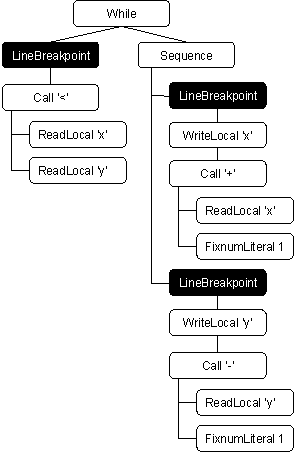
\includegraphics[width=0.7\textwidth]{breakpoints-crop.pdf}
        \label{fig:breakpoints}
      \end{figure}
  \end{columns}


% Idea: Wrapper nodes (e.g. as potendial break point)

% \begin{enumerate}
%  \item Inactive points: define assumptions that they are not activated; truffle optimizes code as the breakpoint would not exists
%  \item Active point: assumption is invalidated, nodes are deopimizated
%  \item On execution: condition is executed, execution may halt; multiple executions triggers again optimization
% \end{enumerate}

% \idea{Zero overhead for inactive or never executed break points}

% \vspace{.3cm}

% Additional: Inline condition \& co for fast debug execution
\end{frame}


\begin{frame}{Debugging (3): Results}
  \begin{figure}
    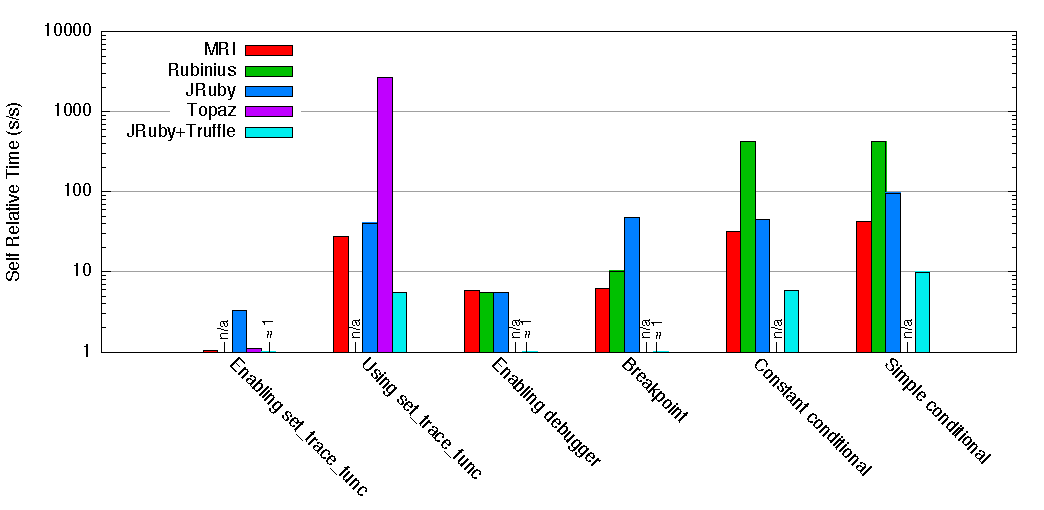
\includegraphics[width=\textwidth]{performance-debugging.pdf}
    \caption{Relative debugging performance in different Ruby VM implementations}
    \label{fig:debuggin_performance}
  \end{figure}
\end{frame}


\section{Summary}
%%%%%%%%%%%%%%%%%

\begin{frame}{Summary}
  Truffle:
  \begin{itemize}
    \item is a framework to write AST interpreters
    \item implements common optimizations - interpreters authors concentrate on implementation domain and language specific specializations and optimizations
    \item results in fast and small interpreter
  \end{itemize}
\end{frame}


\section{References}
%%%%%%%%%%%%%%%%%%%%%%%%%%%%%%%%

\begin{frame}{References}
  \begin{itemize}
    \item C. Seaton, M. L. Van De Vanter, and M. Haupt. Debugging at full speed. In Proceedings of the 8th Workshop on Dynamic Languages and Applications (DYLA), 2014.
    \item T. Würthinger, C. Wimmer, A. Wöß, L. Stadler, G. Duboscq, C. Humer, G. Richards, D. Simon, M. Wolczko. One VM to Rule Them All, 2013.
    \item T. Würthinger, A. Woß, L. Stadler, G. Duboscq, D. Simon, C. Wimmer. Self-Optimizing AST Interpreters, 2012.

    \item Diagrams taken from \emph{One VM to Rule Them All} and \emph{Self-Optimizing AST Interpreters}
  \end{itemize}
\end{frame}

\end{document}
